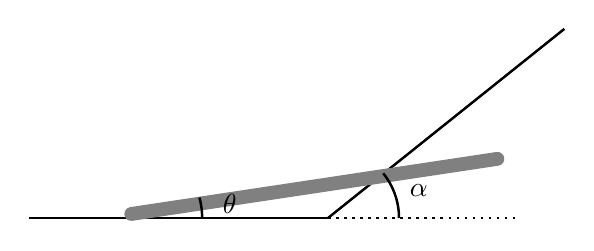
\begin{tikzpicture}[line width=0.9pt]
  % horizontal ground (left flat part)
  \draw (-3.2,0) -- (0.6,0);
  % incline surface going up to the right
  \draw (0.6,0) -- (3.6,2.4);
  % dotted horizontal reference from the kink point
  \draw[dotted] (0.6,0) -- (3.0,0);
  % rod resting between horizontal and incline (thick gray bar)
  \draw[line width=5pt, gray, line cap=round] (-1.9,0.05) -- (2.75,0.75);
  % angle theta between rod and horizontal ground (left)
  \draw (-1.0,0) arc (0:15:1.0);
  \node at (-0.65,0.18) {$\theta$};
  % angle alpha between incline and dotted horizontal (right of kink)
  \draw (1.5,0) arc (0:39:0.9);
  \node at (1.75,0.35) {$\alpha$};
\end{tikzpicture}
